\chapter{RESULTS AND DISCUSSION}

To evaluate the performance and efficiency of our proposed solutions, we developed a comprehensive framework comparing three background subtraction methods—Moving Average, Running Average, and Custom GMM—at original resolution (240×320) with optical flow and data augmentation to reduce false positives and improve generalisation. After identifying Running Average as the most effective, we assessed its impact at different resolutions and measured computational efficiency.

\section{Experimental Setup}

The experiments focused on two primary areas:
\begin{enumerate}
\item Comparing different background subtraction methods (Moving Average, Running Average, and Custom Gaussian Mixture Model)
\item Evaluating the impact of image resolution reduction (240×320, 120×160, 60×80) on model performance
\end{enumerate}

Performance was evaluated using pairwise binary classification accuracy for no-leak (class 0) versus seven leak scenarios (classes 1-7), with the smallest leak size (0-1 pair) being the most challenging and critical for practical applications. Each configuration was evaluated using metrics including accuracy, precision, recall, and F1-score, with particular attention to both leak and no-leak classification performance.

\section{Background Subtraction Methods Comparison}

\subsection{Visual Comparison}

Figure \ref{fig:background_comparison} illustrates the outcomes of various background removal techniques using a class 5 leak scenario. The original infrared frame shows a methane plume with small cloud formations. When processed with different background subtraction techniques, we observe that both Moving Average and our Running Average method better preserve the plume connectivity throughout the structure compared to Custom Gaussian Mixture Model (CGMM). However, all three methods effectively isolate the methane plume from the background.

\begin{figure}[htbp]
\centering
\begin{subfigure}[t]{0.24\textwidth}
\centering
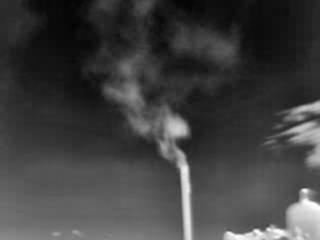
\includegraphics[width=\textwidth]{images/original_frame.png}
\caption{Original infrared frame}
\label{fig:original}
\end{subfigure}%
\hfill%
\begin{subfigure}[t]{0.24\textwidth}
\centering
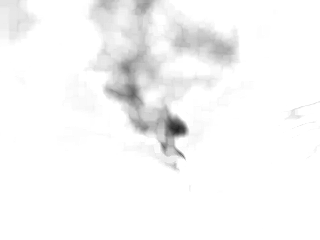
\includegraphics[width=\textwidth]{images/moving_average.png}
\caption{Moving Average}
\label{fig:moving_avg}
\end{subfigure}%
\hfill%
\begin{subfigure}[t]{0.24\textwidth}
\centering
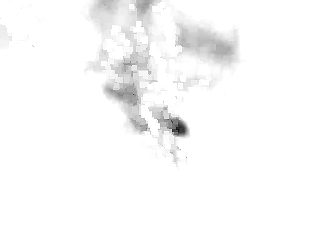
\includegraphics[width=\textwidth]{images/cgmm.png}
\caption{Custom GMM}
\label{fig:cgmm}
\end{subfigure}%
\hfill%
\begin{subfigure}[t]{0.24\textwidth}
\centering
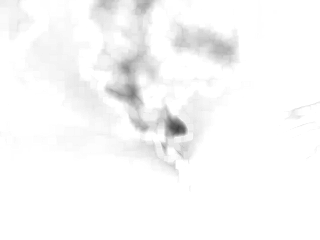
\includegraphics[width=\textwidth]{images/running_average.png}
\caption{Running Average}
\label{fig:running_avg}
\end{subfigure}
\caption{Comparison of background subtraction methods for methane leak detection at 6.9 m distance during class 5 leak duration of GasVid Dataset}
\label{fig:background_comparison}
\end{figure}

\subsection{Overall Classification Performance}

Table \ref{tab:classification_performance} shows the classification metrics for different background subtraction methods, emphasizing precision, recall, and F1-score for both leak and no-leak classes.

\begin{table}[htbp]
\caption{Classification Performance (\%) of Different Background Subtraction Methods}
\label{tab:classification_performance}
\begin{tabular}{|l|c|c|c|c|c|c|c|}
\hline
& \textbf{Overall} & \multicolumn{3}{c|}{\textbf{No-Leak Class}} & \multicolumn{3}{c|}{\textbf{Leak Class}} \\
\cline{3-8}
\textbf{Method} & \textbf{Accuracy} & \textbf{Prec.} & \textbf{Recall} & \textbf{F1} & \textbf{Prec.} & \textbf{Recall} & \textbf{F1} \\
\hline
Running Average & 99.71 & 97.75 & 100 & 98.86 & 100 & 99.67 & 99.84 \\
\hline
Moving Average & 99.58 & 97.05 & 99.69 & 98.35 & 99.95 & 99.57 & 99.76 \\
\hline
Custom GMM & 99.65 & 97.30 & 99.95 & 98.61 & 99.99 & 99.60 & 99.80 \\
\hline
\end{tabular}
\end{table}

The Running Average method achieved the highest overall accuracy at 99.71\%, outperforming both the Moving Average method (99.58\%) and Custom GMM (99.65\%). This improvement, while seemingly marginal, is considerable when combined with the benefits in computational speed.

\subsection{Confusion Matrix Analysis}

The confusion matrices in Table \ref{tab:confusion_matrix} provide insights into the classification performance of each method.

\begin{table}[htbp]
\caption{Confusion Matrix Analysis of Background Subtraction Methods}
\label{tab:confusion_matrix}
\begin{tabular}{|l|c|c|c|c|}
\hline
\textbf{Method} & \textbf{True} & \textbf{False} & \textbf{True} & \textbf{False} \\
& \textbf{No-Leak} & \textbf{No-Leak} & \textbf{Leak} & \textbf{Leak} \\
\hline
Running Average & 1912 & 0 & 13340 & 44 \\
\hline
Moving Average & 1906 & 6 & 13326 & 58 \\
\hline
Custom GMM & 1911 & 1 & 13331 & 53 \\
\hline
\end{tabular}
\end{table}

The Running Average algorithm exhibits perfect performance with zero false positives, a significant improvement over the Custom GMM (1 false positive) and Moving Average algorithm (6 false positives). This elimination of false alarms is critical for field deployment, where false positives can lead to unnecessary inspections and related costs. Additionally, the Running Average method achieves the lowest false negative rate (44) compared to Custom GMM (53) and Moving Average (58), indicating superior sensitivity to actual leaks.

\subsection{Pairwise Classification Performance}

To compare detection performance across different leak sizes, we conducted pairwise comparisons for no-leak (class 0) with each of the leak classes (classes 1-7). Table \ref{tab:pairwise_comparison} provides these results, with emphasis on the challenging 0-1 pair that represents initial leak detection.

\begin{table}[htbp]
\caption{Pairwise Accuracy Comparison (\%) Across Different Background Subtraction Methods}
\label{tab:pairwise_comparison}
\begin{tabular}{|l|c|c|c|c|c|c|c|}
\hline
\textbf{Method} & \textbf{0-1} & \textbf{0-2} & \textbf{0-3} & \textbf{0-4} & \textbf{0-5} & \textbf{0-6} & \textbf{0-7} \\
\hline
Running Average & 98.9 & 100.0 & 100.0 & 100.0 & 100.0 & 100.0 & 99.9 \\
\hline
Moving Average & 98.4 & 99.8 & 99.8 & 99.8 & 99.8 & 99.8 & 99.8 \\
\hline
Custom GMM & 98.6 & 100.0 & 100.0 & 100.0 & 100.0 & 100.0 & 100.0 \\
\hline
\end{tabular}
\end{table}

The Running Average method demonstrates excellent performance on all pairwise comparisons, with perfect 100\% accuracy for most leak classifications (0-2 through 0-6 pairs) and 98.9\% accuracy for the most challenging small leak scenario (0-1 pair), outperforming both Custom GMM (98.6\%) and Moving Average (98.4\%) for this critical case.

\section{Computational Efficiency Analysis}

Table \ref{tab:processing_efficiency} compares the computational efficiency of the background subtraction methods in terms of total video processing time and the average time per frame.

\begin{table}[htbp]
\caption{Computational Efficiency Comparison of Background Subtraction Methods}
\label{tab:processing_efficiency}
\begin{tabular}{|l|c|c|}
\hline
\textbf{Method} & \textbf{Average Video} & \textbf{Average Processing} \\
& \textbf{Processing Time (s)} & \textbf{Time/Frame (ms)} \\
\hline
Running Average & 775.07 & 35.88 \\
Moving Average & 2319.73 & 107.39 \\
Custom GMM & 891.19 & 41.26 \\
\hline
\end{tabular}
\end{table}

The Running Average method is computationally more efficient, taking on average 35.88 ms to process frames, which is approximately 3× faster than the traditional Moving Average method with 210 frames (107.39 ms) and 13\% faster than the Custom GMM (41.26 ms). This speedup in processing is invaluable for real-time applications, where rapid detection enables more immediate responses to leaks.

The improved efficiency stems from the algorithmic simplicity of the Running Average approach—updating the background model requires only the current frame and previous background model, avoiding storing and processing multiple frames. This significantly reduces both memory space and computational complexity without compromising high detection accuracy.

\section{Video Frame Scaling Results}

To assess the feasibility of deploying methane leak detection systems on resource-constrained devices, we experimented with the impact of video frame resolution reduction on model size and detection performance.

\subsection{Model Size Comparison}

Table \ref{tab:model_size_comparison} compares key metrics across three video frame sizes using the Running Average method for background subtraction.

\begin{table}[htbp]
\caption{Model Size Comparison Across Different Video Frame Resolutions}
\label{tab:model_size_comparison}
\begin{tabular}{|l|c|c|}
\hline
\textbf{Video Frame Size} & \textbf{Parameters} & \textbf{Model Size} \\
\hline
240×320×1 & 413,386 (1.58 MB) & 4934 KB \\
120×160×1 & 249,546 (974.79 KB) & 3014 KB \\
60×80×1 & 188,106 (734.79 KB) & 2294 KB \\
\hline
\end{tabular}
\end{table}

Resolution reduction results in dramatic decreases in model parameters and size—the half-resolution model (120×160) requires 39\% fewer parameters than the full-resolution model, while the quarter-resolution model (60×80) requires 55\% fewer parameters. This reduction directly translates to lower memory requirements and computational costs, which are crucial factors for edge deployment.

\subsection{Classification Performance at Reduced Resolutions}

Table \ref{tab:resolution_performance} presents the classification metrics for each resolution using the Running Average background subtraction technique.

\begin{table}[htbp]
\caption{Classification Performance (\%) Across Different Video Resolutions}
\label{tab:resolution_performance}
\setlength{\tabcolsep}{5pt}
\centering
\begin{tabular}{|l|c|c|c|c|c|c|c|}
\hline
\multirow{2}{*}{\textbf{Resolution}} & \textbf{Overall} & \multicolumn{3}{c|}{\textbf{No-Leak Class}} & \multicolumn{3}{c|}{\textbf{Leak Class}} \\
\cline{3-8}
 & \textbf{Accuracy} & \textbf{Prec.} & \textbf{Recall} & \textbf{F1} & \textbf{Prec.} & \textbf{Recall} & \textbf{F1} \\
\hline
240×320 & 99.71 & 97.75 & 100 & 98.86 & 100 & 99.67 & 99.84 \\
\hline
120×160 & 99.27 & 94.78 & 99.63 & 97.14 & 99.95 & 99.22 & 99.58 \\
\hline
60×80 & 98.14 & 87.68 & 99.01 & 93.00 & 99.86 & 98.01 & 98.93 \\
\hline
\end{tabular}
\end{table}


The results show a gradual performance decline as the resolution decreases, with overall accuracy dropping from 99.71\% at full resolution to 99.27\% at half resolution and 98.14\% at quarter resolution. Most significantly, precision on the no-leak class is impacted most with decreased resolution, from 97.75\% at full resolution to 87.68\% at quarter resolution.

Nevertheless, even at quarter resolution, the model achieves over 98\% accuracy in classifying all samples, displaying remarkable robustness to resolution reduction.

\subsection{Pairwise Comparison Across Video Frame Resolutions}

Table \ref{tab:pairwise_resolution} presents the pairwise accuracy comparison for different video frame sizes, highlighting the impact of resolution on detecting leaks of varying sizes.

\begin{table}[htbp]
\caption{Pairwise Accuracy Comparison (\%) Across Different Video Frame Resolutions}
\label{tab:pairwise_resolution}
\begin{tabular}{|l|c|c|c|c|c|c|c|}
\hline
\textbf{Resolution} & \textbf{0-1} & \textbf{0-2} & \textbf{0-3} & \textbf{0-4} & \textbf{0-5} & \textbf{0-6} & \textbf{0-7} \\
\hline
240×320 & 98.9 & 100.0 & 100.0 & 100.0 & 100.0 & 100.0 & 99.9 \\
\hline
120×160 & 97.1 & 99.8 & 99.8 & 99.8 & 99.8 & 99.8 & 99.8 \\
\hline
60×80 & 92.6 & 99.5 & 99.5 & 99.5 & 99.5 & 99.5 & 99.5 \\
\hline
\end{tabular}
\end{table}

The pairwise comparison reveals an important aspect: resolution reduction primarily impacts the detection of small leaks (0-1 pair), where accuracy drops from 98.9\% at full resolution to 97.1\% at half resolution and 92.6\% at quarter resolution. Detection of medium to large leaks (0-2 through 0-7 pairs) is remarkably robust, with accuracy consistently above 99.5\% even at quarter resolution.

This pattern suggests that smaller leaks have more subtle visual patterns that require higher resolution for reliable detection, while larger leaks produce more prominent features that remain detectable even at low resolutions.

\section{Error Analysis}

To provide deeper insights into system limitations and guide practical deployment decisions, we conducted comprehensive error analysis across resolutions using the Running Average method to understand system limitations and guide deployment decisions. Figure \ref{fig:error_analysis} shows representative error cases at different spatial resolutions.

\begin{figure}[htbp]
\centering
\begin{subfigure}[t]{0.31\textwidth}
\centering
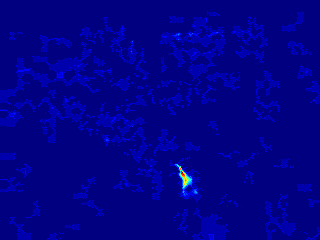
\includegraphics[width=\textwidth]{images/fn_sample_240x320.png}
\caption{False Negative: Subtle leak missed at full resolution}
\label{fig:fn_full}
\end{subfigure}
\hfill
\begin{subfigure}[t]{0.31\textwidth}
\centering
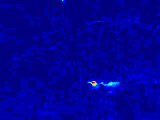
\includegraphics[width=\textwidth]{images/fn_sample_120x160.png}
\caption{False Negative: Small leak detection failure}
\label{fig:fn_half}
\end{subfigure}
\hfill
\begin{subfigure}[t]{0.31\textwidth}
\centering
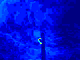
\includegraphics[width=\textwidth]{images/fp_sample_60x80.png}
\caption{False Positive: Background artifact misclassified}
\label{fig:fp_quarter}
\end{subfigure}
\caption{Representative error cases showing detection challenges. (a) Minimal leak signature with low contrast, (b) small leak with dispersed plume pattern, and (c) background noise (windsock) misinterpreted as leak signature.}
\label{fig:error_analysis}
\end{figure}

\subsection{Full Resolution (240×320) Error Analysis}

At full resolution, the system achieved zero false positives with 44 false negatives (0.29\%), primarily from Class 1 scenarios with subtle leak signatures. These missed detections involve minimal visual contrast against background, representing challenging cases for automated detection. The false negative cases typically occur when the methane plume has extremely low density or when environmental conditions (such as wind dispersion) significantly reduce the plume's visual signature.

\subsection{Half-Resolution (120×160) Error Analysis}

The half-resolution model introduced 7 false positives (0.05\%) from misinterpreted background variations and 105 false negatives (0.69\%), mainly affecting small leak detection. Resolution reduction impacts the system's ability to discriminate between subtle leak characteristics and background noise. The increase in false negatives is primarily attributed to the loss of fine-grained spatial details that are crucial for detecting small, dispersed methane plumes.

\subsection{Quarter-Resolution (60×80) Error Analysis}

Error rates increased significantly to 19 false positives (0.12\%) and 266 false negatives (1.74\%) at quarter resolution. False positives demonstrate increased sensitivity to background artifacts when spatial detail is insufficient, while false negatives confirm degraded small leak detection capability. The system begins to misinterpret moving background elements such as windsocks and cloud formations as potential leak signatures due to the reduced spatial resolution.

\subsection{Error Pattern Analysis}

The analysis reveals a clear trade-off between computational efficiency and detection sensitivity:

\begin{enumerate}
\item \textbf{False Negatives:} Primarily occur with minimal leak signatures and dispersed plume patterns that present insufficient visual contrast for reliable detection. These cases represent the fundamental limitation of optical-based detection methods when dealing with extremely subtle gas emissions.

\item \textbf{False Positives:} Occur when background features such as windsock movements or cloud formations are misinterpreted as leak signatures, particularly at reduced resolutions where spatial detail is insufficient for proper discrimination.

\item \textbf{Resolution Impact:} Full resolution ensures maximum sensitivity for safety-critical applications, while half resolution provides optimal balance for medium-to-large leak detection with reduced computational overhead.
\end{enumerate}

\section{Discussion}

\subsection{Background Subtraction Method Performance}

The comparative analysis across different background subtraction methods reveals several key insights:

\begin{enumerate}
\item \textbf{Superior Accuracy:} The Running Average method achieved the highest overall accuracy (99.71\%) with exceptional precision for leak detection (100\%) and the lowest false positive rate.

\item \textbf{Computational Efficiency:} The Running Average method demonstrated the best computational efficiency with 3× faster processing compared to Moving Average, making it suitable for real-time applications.

\item \textbf{Adaptive Capability:} The dynamic background modeling capability of Running Average effectively accounts for gradual changes in environmental conditions.
\end{enumerate}

\subsection{Resolution Trade-offs}

The study revealed important insights regarding the relationship between image resolution and detection performance:

\begin{enumerate}
\item \textbf{Optimal Balance:} Half-resolution (120×160) images offer a favorable balance between computational efficiency and detection accuracy, with only 0.44\% accuracy decrease.

\item \textbf{Leak Size Dependency:} The impact of resolution reduction is highly dependent on leak size, with small leaks being more affected than larger ones.

\item \textbf{Practical Deployment:} Quarter-resolution models maintain excellent performance for medium to large leaks while maximizing computational efficiency.
\end{enumerate}

\subsection{Practical Implications}

The findings have significant implications for real-world deployment:

\begin{enumerate}
\item \textbf{Real-time Capability:} The 3× improvement in processing speed enables real-time monitoring in industrial environments.

\item \textbf{Cost-effective Implementation:} Zero false positives reduce unnecessary inspections and operational costs.

\item \textbf{Edge Device Deployment:} Model size reduction of up to 55\% enables deployment on resource-constrained devices.

\item \textbf{Scalable Solutions:} The optimized approach can be scaled across multiple monitoring points in industrial facilities.
\end{enumerate}